\documentclass[journal,12pt,twocolumn]{IEEEtran}

\usepackage{setspace}
\usepackage{gensymb}
\usepackage[cmex10]{amsmath}
\usepackage{tikz}
\usetikzlibrary{automata,positioning}
\usepackage{amsthm}
\usepackage{amsmath}
\usepackage{blkarray}
\usepackage{mathrsfs}
\usepackage{txfonts}
\usepackage{stfloats}
\usepackage{bm}
\usepackage{cite}
\usepackage{cases}
\usepackage{subfig}

\usepackage{longtable}
\usepackage{multirow}

\usepackage{enumitem}
\usepackage{mathtools}
\usepackage{steinmetz}

\usepackage{circuitikz}
\usepackage{verbatim}
\usepackage{tfrupee}
\usepackage[breaklinks=true]{hyperref}
\usepackage{graphicx}
\usepackage{tkz-euclide}

\usetikzlibrary{calc,math}
\usepackage{listings}
    \usepackage{color}                                            %%
    \usepackage{array}                                            %%
    \usepackage{longtable}                                        %%
    \usepackage{calc}                                             %%
    \usepackage{multirow}                                         %%
    \usepackage{hhline}                                           %%
    \usepackage{ifthen}                                           %%
    \usepackage{lscape}     
\usepackage{multicol}
\usepackage{chngcntr}

\DeclareMathOperator*{\Res}{Res}

\renewcommand\thesection{\arabic{section}}
\renewcommand\thesubsection{\thesection.\arabic{subsection}}
\renewcommand\thesubsubsection{\thesubsection.\arabic{subsubsection}}

\renewcommand\thesectiondis{\arabic{section}}
\renewcommand\thesubsectiondis{\thesectiondis.\arabic{subsection}}
\renewcommand\thesubsubsectiondis{\thesubsectiondis.\arabic{subsubsection}}


\newcommand{\define}{\stackrel{\triangle}{=}}


\theoremstyle{definition}
\newtheorem{definition}{Definition}[section]
\newtheorem{theorem}{Theorem}[section]
\newtheorem{lemma}[theorem]{Lemma}
\newtheorem*{remark}{Remark}

\bibliographystyle{IEEEtran}
\raggedbottom
\setlength{\parindent}{0pt}
\providecommand{\mbf}{\mathbf}
\providecommand{\pr}[1]{\ensuremath{\Pr\left(#1\right)}}
\providecommand{\qfunc}[1]{\ensuremath{Q\left(#1\right)}}
\providecommand{\sbrak}[1]{\ensuremath{{}\left[#1\right]}}
\providecommand{\lsbrak}[1]{\ensuremath{{}\left[#1\right.}}
\providecommand{\rsbrak}[1]{\ensuremath{{}\left.#1\right]}}
\providecommand{\brak}[1]{\ensuremath{\left(#1\right)}}
\providecommand{\lbrak}[1]{\ensuremath{\left(#1\right.}}
\providecommand{\rbrak}[1]{\ensuremath{\left.#1\right)}}
\providecommand{\cbrak}[1]{\ensuremath{\left\{#1\right\}}}
\providecommand{\lcbrak}[1]{\ensuremath{\left\{#1\right.}}
\providecommand{\rcbrak}[1]{\ensuremath{\left.#1\right\}}}

\newcommand{\sgn}{\mathop{\mathrm{sgn}}}
\providecommand{\abs}[1]{\vert#1\vert}
\providecommand{\res}[1]{\Res\displaylimits_{#1}} 
\providecommand{\norm}[1]{\lVert#1\rVert}
%\providecommand{\norm}[1]{\lVert#1\rVert}
\providecommand{\mtx}[1]{\mathbf{#1}}
\providecommand{\mean}[1]{E[ #1 ]}
\providecommand{\fourier}{\overset{\mathcal{F}}{ \rightleftharpoons}}
%\providecommand{\hilbert}{\overset{\mathcal{H}}{ \rightleftharpoons}}
\providecommand{\system}{\overset{\mathcal{H}}{ \longleftrightarrow}}
	%\newcommand{\solution}[2]{\textbf{Solution:}{#1}}
\newcommand{\solution}{\noindent \textbf{Solution: }}
\newcommand{\cosec}{\,\text{cosec}\,}
\providecommand{\dec}[2]{\ensuremath{\overset{#1}{\underset{#2}{\gtrless}}}}
\newcommand{\myvec}[1]{\ensuremath{\begin{pmatrix}#1\end{pmatrix}}}
\newcommand{\mydet}[1]{\ensuremath{\begin{vmatrix}#1\end{vmatrix}}}
\numberwithin{equation}{subsection}
\makeatletter
\@addtoreset{figure}{problem}
\makeatother
\let\StandardTheFigure\thefigure
\let\vec\mathbf
\renewcommand{\thefigure}{\theproblem}
\def\putbox#1#2#3{\makebox[0in][l]{\makebox[#1][l]{}\raisebox{\baselineskip}[0in][0in]{\raisebox{#2}[0in][0in]{#3}}}}
     \def\rightbox#1{\makebox[0in][r]{#1}}
     \def\centbox#1{\makebox[0in]{#1}}
     \def\topbox#1{\raisebox{-\baselineskip}[0in][0in]{#1}}
     \def\midbox#1{\raisebox{-0.5\baselineskip}[0in][0in]{#1}}

\lstset{
frame=single, 
breaklines=true,
columns=fullflexible
}
\begin{document}
\title{Assignment 3}
\author{Vibhavasu Pasumarti - EP20BTECH11015}
\maketitle
\newpage
\bigskip
\renewcommand{\thefigure}{\theenumi}
\renewcommand{\thetable}{\theenumi}
Download all python codes from 
\begin{lstlisting}
https://github.com/VIB2020/AI1103/blob/main/Assignment%203/code/Assignment%203.py
\end{lstlisting}
and latex-tikz codes from 
\begin{lstlisting}
https://github.com/VIB2020/AI1103/blob/main/Assignment%203/Assignment%203.pdf
\end{lstlisting}
\section{\large GATE 2015 (EE paper 01 new 2), Q 27 (Electrical Engg section)}
Two players A, and B alternately keep rolling a fair dice. The person to get a six first wins the game. Given that player A starts the game, the probability that A wins the game is:\\[5pt]
    A $\dfrac{5}{11}$ \hspace{1cm}
    B $\dfrac{1}{2}$ \hspace{1cm}
    C $\dfrac{7}{13}$ \hspace{1cm}
    D $\dfrac{6}{11}$ \hspace{1cm}
\section{\Large Solution}
\begin{itemize}
    \item Given the die is fair.
    \item So, for any given throw by A or B:\\
    The probability of getting 6 = $\dfrac{1}{6}$ = p (say)\\
    The probability of NOT getting 6 = $\dfrac{5}{6}$ = q (say)
\end{itemize}
\begin{figure}[h]
    \centering
    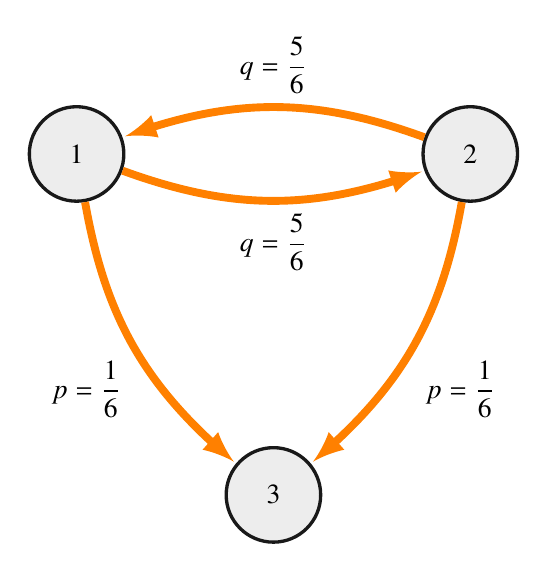
\begin{tikzpicture}[roundnode/.style={circle, draw=black!90, fill=black!7, very thick, minimum size=1.2cm}]
        \node [roundnode] at (0, 0)     (a)     {1};
        \node [roundnode] at (5, 0)     (b)     {2};
        \node [roundnode] at (2.5, -4.3301) (w) {3};
        \draw[every loop, auto=right, line width=1mm,
                >=latex, draw=orange,fill=orange]
            (a) edge[bend right=20] node {$q = \dfrac{5}{6}$} (b)
            (b) edge[bend right=20] node {$q = \dfrac{5}{6}$} (a)
            (a) edge[bend right=20] node {$p = \dfrac{1}{6}$} (w)
            (b) edge[bend left=20, auto=left] node {$p =     \dfrac{1}{6}$} (w);
    \end{tikzpicture}
        \caption{Markov chain for the given problem}
        \label{fig:my_label}
\end{figure}
    
\begin{center}
    \begin{tabular}{|c|c|}
        \hline
        State & Corresponding description \\
        \hline
        \multirow{ 2}{*}{1} & Player who plays first.\\
        & Here: PLAYER A\\
        \hline
        \multirow{ 2}{*}{2} & Player who plays second.\\
        & Here: PLAYER B\\
        \hline
        3 & WINNER\\
        \hline
        \multicolumn{2}{c}{Table 1: State description table}
    \end{tabular}
\end{center}
\begin{definition}
    Transition/Stochastic matrix corresponding to single throw of dice: X\\
    \centering
         \text{\small (From)} \begin{blockarray}{ *{4}{c} }
                \multicolumn{3}{c}{(\small To)}\\
                & 1 & 2 & 3 \\
                \begin{block}{ c @{\quad} [ @{\,} *{3}{c} @{\,} ] }
                    1 & 0 & q & p\\ 
                    2 & q & 0 & p\\
                    3 & 0 & 0 & 0\\
                \end{block}
           \end{blockarray} = X\\
           $X^n$ corresponds to n throws of dice
    \begin{align}
            \pr{\text{A wins in 'i' throws}} = p_{13}(i) = (X^i)_{13} 
    \end{align}
\end{definition}
\begin{lemma} \large
    \begin{align}
        \lim_{n \to \infty}p_{13}(n) = 0
    \end{align}
\end{lemma}
\begin{proof}
   \begin{align}
        p , q < 1
        \implies \text{X is reducible.}\\
        \implies \lim_{n \to \infty} (X)^n \to 0\label{Eqn:2.1}\\
        \lim_{n \to \infty}{(X)^n}_{13} = 0
        \therefore \lim_{n \to \infty} p_{13}(n) = 0
    \end{align}
\end{proof}
\begin{align}
    \intertext{Given: A throws first.}
    \implies p_{13}(1) = X_{13} = p 
    \intertext{After second throw: (by B)}
    X^2 = \myvec{0 & q & p\\ q & 0 & p\\ 0 & 0 & 0} \myvec{0 & q & p\\ q & 0 & p\\ 0 & 0 & 0}\\
    = \myvec{ 0 & 0 & 0\\0 & q^2 & qp\\0 & 0 & 0}
    \implies  p_{13}(2) = 0\\
    X^3 = \myvec{ 0 & q & p\\0 & 0 & 0\\0 & 0 & 0}\myvec{ 0 & 0 & 0\\0 & q^2 & qp\\0 & 0 & 0}\\
    =\myvec{ 0 & q^3 & q^2p\\0 & 0 & 0\\0 & 0 & 0}
    \implies  p_{13}(3) = q^2 p
\end{align}
\centering \begin{tabular}{|c|c|}
    \hline\
    $p_{13}(i)$ & Probability \\
    \hline
    $p_{13}(1)$ & $p$ = 1/6\\
    \hline
    $p_{13}(2)$ & 0\\
    \hline
    $p_{13}(3)$ & $q^2p$\\
    \hline
    \vdots & \vdots\\
    $p_{13}(2n)$ & 0\\
    \hline
    $p_{13}(2n + 1)$ & $q^{2n}p$\\
    \hline
    \multicolumn{2}{c}{Table 2: Summary of Probabilities}\\
\end{tabular}
\onehalfspacing
\begin{align}
    \pr{\text{A wins}} = \sum_{n=1}^{\infty} p_{13}(n)\\
    = p + 0 + q^2p + 0 + q^4p + ....\\
    = \sum_{k=1}^{\infty} (q^2)^k p
    = p \sum_{k=1}^{\infty} (q^2)^k \hspace{0.5cm} \text{But $|q| <$ 1}\\
    = p \left(\dfrac{1}{1 - q^2}\right)
    =\dfrac{\frac{1}{6}}{1 - \frac{25}{36}} = \dfrac{6}{11}
\end{align}
\centering \Large
\pr{\text{A wins the game}} = $\dfrac{6}{11}$\\
Option D is correct
\end{document}
